
\chapter{Implementierung der DSL}

\section{Lexer \& Parser}
Lexer und Parser werden beide von einer ANTLR4 Grammatik erzeugt.

\section{Abstrakter Syntaxbaum}
Ein \ac{AST} ist ein Baum, der bei dem Parsen der \ac{DSL} aufgebaut wird.
Dieser wird anschließend von dem Interpreter abgearbeitet / ausgeführt.\\
Der Baum besteht aus Knoten, die in einer Baumstruktur an einer Wurzel hängen.
In PrePro gibt es eine Vielzahl an verschiedener Knoten-Typen.\\
Die Klassenhierarchie ist in \abb{fig:NodesHierachy} abgebildet.
Als oberstes Element ist das Interface \texttt{PreProNode} definiert.
Die \texttt{MainNode} ist der Wurzelknoten des \ac{AST}.

\begin{figure}
	\centering
	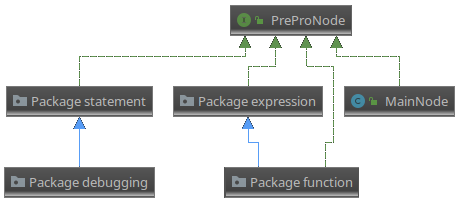
\includegraphics[width=\textwidth]{figures/uml_nodes}
	\caption{Die Knoten-Klassenhierarchie}
	\label{fig:NodesHierachy}
\end{figure}

\begin{figure}
	\centering
	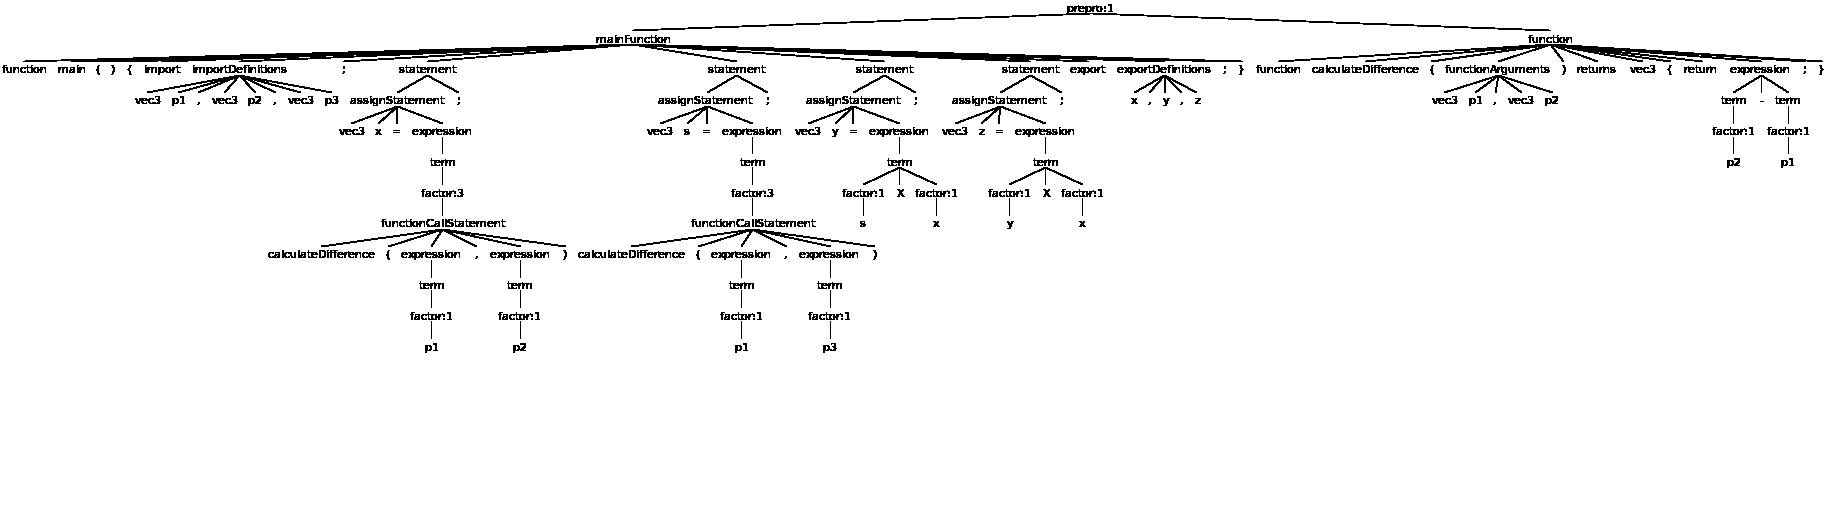
\includegraphics[width=\textwidth]{figures/parseTree}
	\caption{Beispielhafter \ac{AST}}
	\label{fig:AST}
\end{figure}

\section{Typsystem}
\begin{figure}
	\centering
	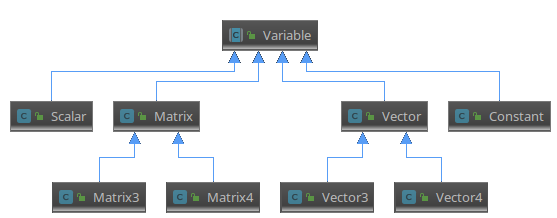
\includegraphics[width=\textwidth]{figures/typsystem}
	\caption{Typsystem von PrePro}
	\label{fig:Typsystem}
\end{figure}
Das Typsystem von PrePro ist in \abb{fig:Typsystem} dargestellt.
Alle Variablen erben von er abstrakten Klasse \texttt{Variable}.
Es gibt die Untertypen \texttt{Vector}, \texttt{Marix}, \texttt{Scalar} und \texttt{Constant}.
Die Unterklassen \texttt{Vector} und \texttt{Matrix} haben wiederum Unterklassen für drei- und vierelementige Varianten.
Diese Unterklassen sind wichtig, da z.B. eine \texttt{Matrix3} mit einem \texttt{Vector3} multipliziert werden kann, allerdings nicht mit einem \texttt{Vector4}.\\
In der abstrakten Klasse \texttt{Variable} sind die Funktionen \texttt{add}, \texttt{sub}, \texttt{mul} und \texttt{div} definiert.
Werden die Funktionen auf der abstrakten Klasse aufgerufen, werfen sie eine Exception, dass die mathematische Operation nicht definiert sei.\\
Die Unterklassen haben nun die Möglichkeit, Operationen mit anderen Typen zu definieren.
Mittels Polymorphie und dynamic dispatching wird bei einer arithmetischen Operation die passende Funktion gesucht.
Falls keine passende Funktion wird die allgemeine - in der abstrakten Klasse definierte - Funktion verwendet, und daraufhin eine Exception geworfen, dass die mathematische Operation nicht definiert sei.

\subsection{Darstellung der Typen in Java}
Alle Typen werden als \texttt{INDArray} von \texttt{ND4J} dargestellt.\\
Die Unterklassen besitzen einen Konstruktor, der ein \texttt{INDArray} übergeben bekommt.
In den Konstruktoren wird jeweils geprüft, ob die Dimensionen dem entsprechenden Typ entsprechen (z.B eine Matrix4 muss eine 4x4-Matrix übergeben bekommen).
Die einzige Ausnahme bildet der Typ ``Constant'', dieser bietet zusätzlich einen Konstruktur, dem ein \texttt{double} übergeben werden kann.
Intern wird aus dem \texttt{double} ein \texttt{INDArray} erzeugt.

\section{FunctionTable}

\section{SymbolTable}

\section{Grundrechenarten}
Bei der Darstellung der Zahlen im Speicher wird für jede Zahl ein Double verwendet.
Das erhöht die Genauigkeit gegenüber einem float und erspart Konvertierungen zwischen Ganz- und Fließzahlen.
Grundrechenarten sind die Addition, Subtraktion, Multiplikation und Division von Matrizen.
Sie Operationen sind elementweise und werden direkt von ND4J zur Verfügung gestellt und können aufgerufen werden.

\section{Kreuzprodukt}
Anders als die vier Grundarten aus dem vorherigen Abschnitt wird das Kreuzprodukt von ND4J nicht als Operation angeboten.
Das Kreuzprodukt wird in der Praxis allerdings zu Beispiel für das Aufspannen von Vektoren im dreidimensionalen Raum benötigt.
Daher wird an dieser Stelle das Kreuzprodukt zweier Vektoren selber implementiert.
Falls ND4J in Zukunft den Operator Kreuzprodukt bereit stellt, kann in zukünftigen Varianten auf ihre Implementierung zugegriffen werden, da diese wahrscheinlich effizienter sein wird.
Die eigene Implementierung des Kreuzprodukts kann auf folgende Arten geschehen:
\begin{enumerate}
	\item Implementierung in Plain Java mittels einer for-Schleife.
	\item Implementierung in Plain Java mittels Subarrays
\end{enumerate}

\subsection{Implementierung Kreuzprodukt mittels For-Schleife}
Bei der Implementierung mittels der For-Schleife werden die eigentlichen Berechnungen in Java durchgeführt.
Als erstes wird ein Double-Array als Zwischenspeicher für das Ergebnis angelegt.
Es besitzt (Anzahl der Zeitelemente in den Eingabe-Vektoren) * drei Elemente.
Die Anzahl der Elemente entspricht so der Anzahl der Elemente der Ergebnismatrix, die Daten können in dem Double-Array effizient gespeichert werden.
Das Array wird im Anschluss in eine Matrix konvertiert.
Für die Berechnung der Elemente wird mittels einer For-Schleife über alle Zeilen der Matrix iteriert.
In jeder Zeile werden die 3 Werte des entstehenden Ergebnisvektors berechnet und in das Double-Array gespeichert.
Abschließend wir das Double-Array in eine Matrix mit den Dimensionen [<Anzahl Zeitelemente> x drei] konvertiert und durch eine Vector3-Wrapper-Klasse als Vector mit 3 Werten gekennzeichnet.
Der Algorithmus ist in \code{lst:Kreuzprodukt_For} dargestellt.
\\\\
\begin{minipage}{\linewidth}
\begin{lstlisting}[language=java, label={lst:Kreuzprodukt_For}, caption={Implementierung Kreuzprodukt mittels for-Schleife}, captionpos=b]
private Vector3 crossProduct(Vector3 left, Vector3 right) {
    INDArray a = left.getNdArray();
    INDArray b = right.getNdArray();

    int size = a.shape()[0];
    double[] result = new double[size * 3];

    for (int i = 0; i < size; i++) {
        result[i * 3 + 0] = a.getDouble(i, 1) * b.getDouble(i, 2) - a.getDouble(i, 2) * b.getDouble(i, 1);
        result[i * 3 + 1] = a.getDouble(i, 2) * b.getDouble(i, 0) - a.getDouble(i, 0) * b.getDouble(i, 2);
        result[i * 3 + 2] = a.getDouble(i, 0) * b.getDouble(i, 1) - a.getDouble(i, 1) * b.getDouble(i, 0);
    }
    return new Vector3(Nd4j.create(result, new int[]{size, 3}));
}
\end{lstlisting}
\end{minipage}

\subsection{Implementierung Kreuzprodukt mittels Subarrays}
\begin{minipage}{\linewidth}
\begin{lstlisting}[language=java, label={lst:Kreuzprodukt_Subarray}, caption={Implementierung Kreuzprodukt mittels for-Schleife}, captionpos=b]
private Vector3 crossProductSubArray(Vector3 left, Vector3 right) {
    INDArray a = left.getNdArray();
    INDArray b = right.getNdArray();

    INDArray a1 = a.getColumn(0);
    INDArray a2 = a.getColumn(1);
    INDArray a3 = a.getColumn(2);

    INDArray b1 = b.getColumn(0);
    INDArray b2 = b.getColumn(1);
    INDArray b3 = b.getColumn(2);

    INDArray c1 = (a2.mul(b3)).sub(a3.mul(b2));
    INDArray c2 = (a3.mul(b1)).sub(a1.mul(b3));
    INDArray c3 = (a1.mul(b2)).sub(a2.mul(b1));

    int size = a.shape()[0];
    INDArray result = Nd4j.create(size, 3);
    result.putColumn(0, c1);
    result.putColumn(1, c2);
    result.putColumn(2, c3);

    return new Vector3(result);
}
\end{lstlisting}
\end{minipage}

\section{Vergleich der Implementierungen für Kreuzprodukt}
Beide Impelemtierungsmöglichkeiten haben Vor- und Nachteile.
Diese sind in \tab{tab:Vorteile_Kreuzprodukt_Implementierungen} aufgeführt.
\begin{table}[H]
	\centering
	\begin{tabular}{ | p{4cm} | p{5.5cm} | p{5.5cm} | }
		\hline \rowcolor{gray!15}
		\textbf{Implementierungs-möglichkeit} & \textbf{Vorteile} & \textbf{Nachteile} \\ \hhline{|=|=|=|}
		Mittels For-Schleife & Leichter verständlich. & Wird direkt in Java ausgeführt. \newline Mögliche Optimierungen von ND4J können nicht verwendet werden. Berechnungen finden nur auf der \ac{CPU} statt! \\ \hline
		Mittels Subarray & Durch die Verwendung von ND4J können die Optimierungen verwendet werden. Wenn ND4J so konfiguriert ist, dass es auf der \ac{GPU} läuft, kann die eigentliche Berechnung weiterhin auf der \ac{GPU} erfolgen. & Schwerer verständlich. \\ \hline
	\end{tabular}
	\caption{Vor- und Nachteile einer Implementierung mittels Compiler oder Interpreter}
	\label{tab:Vorteile_Kreuzprodukt_Implementierungen}
\end{table}

\noindent Für große Zeitreihen müsste sich die Implementierung mittels dem Subarray als effizienter erweisen, besonders wenn die Berechnungen auf der \ac{GPU} durchgeführt werden.
Als Nachweis und für das Effizienzverhalten bei kleinen Zeitreihen wurde ein Benchmark durchgeführt.
Die Ergebnisse sind in \tab{tab:Benchmark_Kreuzprodukt_Implementierung} festgehalten.

\begin{table}[H]
	\centering
	\begin{tabular}{ | p{5cm} | p{3.5cm} | p{3.5cm} | }
		\hline \rowcolor{gray!15}
		\textbf{Anzahl Datensätze} & \textbf{For-Schleife} & \textbf{Subarray} \\ \hhline{|=|=|=|}
		100 & 6 (342) & 4 (13) \\ \hline
		1.000 & 20 (489) & 7 (22) \\ \hline
		10.000 & 53 (527) & 5 (21) \\ \hline
		100.000 & 333 (1159) & 5 (15) \\ \hline
		1.000.000 & 3205 (4129) & 47 (64) \\ \hline
		10.000.000 & 32358 (33594) & 442 (453) \\ \hline

	\end{tabular}
	\caption{Benchmark-Ergebnisse in ms der verschiedenen Implementierungsmöglichkeiten für das Kreuzprodukt. Die Messung ist nach 5 Durchläufen gemessen, die Zahl in Klammern gibt die Zeit des ersten Durchlaufs an.}
	\label{tab:Benchmark_Kreuzprodukt_Implementierung}
\end{table}

3 Varianten

Benchmarks!
Klassifizierung \ac{CPU} oder \ac{GPU}-Workload.

Möglicherweise lohnt sich die eher \ac{GPU}-betonte Variante erst ab gewisser Größe.
=> Dann mit konstantem Aufwand entscheiden, welches Verfahren.
Vom Nutzer (während Laufzeit) auswählbar?
%%%%%%%%%%%%%%%%%%%%%%%%%%%%%%%%%%%%%%%%%%%%%%%%%%%%%%%%%%%%%%%%%%%%%%%%%%%%%%%
\endinput
%%%%%%%%%%%%%%%%%%%%%%%%%%%%%%%%%%%%%%%%%%%%%%%%%%%%%%%%%%%%%%%%%%%%%%%%%%%%%%%
